\documentclass[12pt]{article}


\usepackage{amssymb}
\usepackage{amsmath}
\usepackage{fullpage}
\usepackage{epsfig}
\usepackage{epstopdf}
\everymath{\displaystyle}
\usepackage{enumerate}

\newif\ifans

\anstrue

\begin{document}

\begin{center}
\underline{\LARGE{Chapter 3.9: Inverse Trigonometric Functions}}
\end{center}

\subsection*{Expected Skills:}

\begin{itemize}

\item Be able to specify the domain and range of $\sin^{-1}(x)$, $\cos^{-1}(x)$, and $\tan^{-1}(x)$.  Also be able to graph these functions.

\item Be able to evaluate an inverse trigonometric function at a ratio which is related to the common angles of $0^\circ-30^\circ-45^\circ-60^\circ-90^\circ$.

\item Be able to evaluate limits involving inverse trigonometric functions.

\item Be able to differentiate $\sin^{-1}(x)$, $\cos^{-1}(x)$, and $\tan^{-1}(x)$.  Also be able to use the derivative to solve application problems.

\end{itemize}

\subsection*{Practice Problems: }

\begin{enumerate}

\item For each of the following functions, state the domain and the range.

\begin{enumerate}

\item $\displaystyle f(x)=\sin^{-1}{x}$

\ifans \fbox{Domain: $[-1,1]$, Range: $\displaystyle \left[-\frac{\pi}{2},\frac{\pi}{2}\right]$} \fi

\item $\displaystyle f(x)=\cos^{-1}{x}$

\ifans \fbox{Domain: $[-1,1]$, Range: $\displaystyle [0,\pi]$} \fi

\item $\displaystyle f(x)=\tan^{-1}{x}$

\ifans \fbox{Domain: $(-\infty,\infty)$, Range: $\displaystyle \left(-\frac{\pi}{2},\frac{\pi}{2}\right)$} \fi

\end{enumerate}

\item Evaluate each of the following. (Do not use a calculator.  And remember the ranges from problem 1.)

\begin{enumerate}

\item $\displaystyle \arcsin{\frac{\sqrt{3}}{2}}$

\ifans \fbox{$\displaystyle \frac{\pi}{3}$} \fi

\item $\displaystyle \arcsin{\left(-\frac{\sqrt{3}}{2}\right)}$

\ifans \fbox{$\displaystyle -\frac{\pi}{3}$} \fi

\item $\displaystyle \arccos{\frac{\sqrt{3}}{2}}$

\ifans \fbox{$\displaystyle \frac{\pi}{6}$} \fi

\item $\displaystyle \arccos{\left(-\frac{\sqrt{3}}{2}\right)}$

\ifans \fbox{$\displaystyle \frac{5\pi}{6}$} \fi

\item $\displaystyle \arctan{\frac{\sqrt{3}}{3}}$ 

\ifans \fbox{$\displaystyle \frac{\pi}{6}$} \fi

\item $\displaystyle \arctan{\left(-\frac{\sqrt{3}}{3}\right)}$ 

\ifans \fbox{$\displaystyle -\frac{\pi}{6}$} \fi

\end{enumerate}

\item Use an inverse trigonometric function to express $\theta$ as a function of $x$:

\begin{tabular}{ll}

(a) \setlength{\unitlength}{.4in}
\begin{picture}(7,5)(0,0)
\linethickness{1pt}
\put(0,0){\line(1,0){4}}
\put(4,0){\line(0,1){3}}
\put(0,0){\line(4,3){4}}
\put(2,-.25){\makebox(0,0){$4$}}
\put(4.25,1.5){\makebox(0,0){$x$}}
%\put(2,2){\makebox(0,0){$9$}}
\put(0.7,0.2){\makebox(0,0){$\theta$}}
\end{picture}

&

(b) 
\setlength{\unitlength}{.4in}
\begin{picture}(7,5)(0,0)
\linethickness{1pt}
\put(0,0){\line(1,0){4}}
\put(4,0){\line(0,1){3}}
\put(0,0){\line(4,3){4}}
\put(2,-.25){\makebox(0,0){$x+3$}}
%\put(4.25,1.5){\makebox(0,0){$30$}}
\put(2,2){\makebox(0,0){$2x$}}
\put(0.7,0.2){\makebox(0,0){$\theta$}}
\end{picture}

\end{tabular}

\bigskip

\ifans \fbox{(a) $\displaystyle \theta=\tan^{-1}{\left(\frac{x}{4}\right)}$, (b) $\displaystyle \theta=\cos^{-1}{\left(\frac{x+3}{2x}\right)}$} \fi

\item Find the exact value of each expression. 

\begin{enumerate}

\item $\displaystyle \sin{\left(\tan^{-1}{\left(\frac{3}{4}\right)}\right)}$

\ifans\fbox{$\displaystyle \frac{3}{5}$}\fi

\item $\displaystyle \sec{\left(\arctan{\left(-\frac{3}{5}\right)}\right)}$

\ifans\fbox{$\displaystyle \frac{\sqrt{34}}{5}$}\fi

\item $\displaystyle \sin{\left(\arccos{\left(-\frac{2}{3}\right)}\right)}$

\ifans\fbox{$\displaystyle \frac{\sqrt{5}}{3}$}\fi

\item $\displaystyle \csc{\left(\cos^{-1}{\left(\frac{\sqrt{3}}{2}\right)}\right)}$

\ifans\fbox{$2$}\fi

\end{enumerate}

\item Find the exact value of each expression.  Remember the ranges from problem (1)!

\begin{enumerate}

\item $\displaystyle \sin^{-1}{\left(\sin{\left(\frac{\pi}{3}\right)}\right)}$

\ifans\fbox{$\displaystyle \frac{\pi}{3}$}\fi

\item $\displaystyle \sin^{-1}{\left(\sin{\left(\frac{2\pi}{3}\right)}\right)}$

\ifans\fbox{$\displaystyle \frac{\pi}{3}$}\fi

\item $\displaystyle \cos^{-1}{\left(\cos{\left(\frac{\pi}{4}\right)}\right)}$

\ifans\fbox{$\displaystyle \frac{\pi}{4}$}\fi

\item $\displaystyle \cos^{-1}{\left(\cos{\left(-\frac{\pi}{4}\right)}\right)}$

\ifans\fbox{$\displaystyle \frac{\pi}{4}$}\fi

\item $\displaystyle \tan^{-1}{\left(\tan{\left(\frac{\pi}{6}\right)}\right)}$

\ifans\fbox{$\displaystyle \frac{\pi}{6}$}\fi

\item $\displaystyle \tan^{-1}{\left(\tan{\left(\frac{5\pi}{6}\right)}\right)}$

\ifans\fbox{$\displaystyle -\frac{\pi}{6}$}\fi

\end{enumerate}

\item For each of the following, find all solutions in the interval $[0,2\pi]$.  Give the exact values, not decimal approximations.

\begin{enumerate}

\item $(\sin{x}-1)(4\sin{x}-3) = 0$

\ifans\fbox{$\frac{\pi}{2}$, $\arcsin\left(\frac{3}{4}\right)$, $\pi-\arcsin\left(\frac{3}{4}\right)$} \fi

\item $3\tan{x}=1$

\ifans \fbox{$\tan^{-1}\left(\frac{1}{3}\right)$, $\pi+\tan^{-1}\left(\frac{1}{3}\right)$} \fi

\item $5\cos^2{x}+11\cos{x}+2=0$

\ifans \fbox{\parbox{1\linewidth}{
Notice that solving this equation reduces to solving $\cos{x}=-\frac{1}{5}$.  So, there are solutions in both quadrants II and III.  The reference angle is $\arccos\left(\frac{1}{5}\right)$.  Thus, the two solutions of the given equation are $\pi - \arccos\left(\frac{1}{5}\right)$ and $\pi + \arccos\left(\frac{1}{5}\right)$.\\
\\
Alternatively, one could find the angle in the second quadrant by calculating $\arccos\left(-\frac{1}{5}\right)$.  Then, the angle in the third quadrant is $2\pi-\arccos\left(-\frac{1}{5}\right)$}} \fi

\item $3\tan{x}=-1$

\ifans \fbox{$\pi+\tan^{-1}\left(-\frac{1}{3}\right)$, $2\pi+\tan^{-1}\left(-\frac{1}{3}\right)$} \fi

\end{enumerate}

\item Evaluate the following limits.  If a limit does not exist, write $+\infty$, $-\infty$, or DNE.

\begin{enumerate}

\item $\displaystyle \lim_{x\rightarrow \infty}{\arccos{\left(\frac{-x^2}{x^2+3x}\right)}}$ 

\ifans{\fbox{$\displaystyle \pi$}} \fi

\item $\displaystyle \lim_{x\rightarrow 0}{\arctan{\left(\frac{1}{x^2}\right)}}$ 

\ifans{\fbox{$\displaystyle \frac{\pi}{2}$}} \fi

\item $\lim_{h \rightarrow 0}{\frac{\sin^{-1}{\left(\frac{\sqrt{3}}{2}+h\right)}-\frac{\pi}{3}}{h}}$ \\({\bf Hint:} Interpreting the limit as the derivative of a function a particular point.)

\ifans{\fbox{$\lim_{h \rightarrow 0}{\frac{\sin^{-1}{\left(\frac{\sqrt{3}}{2}+h\right)}-\frac{\pi}{3}}{h}}=\left.\frac{d}{dx}(\sin^{-1}{(x)}\right|_{x=\frac{\sqrt{3}}{2}}=\left.\frac{1}{\sqrt{1-x^2}}\right|_{x=\frac{\sqrt{3}}{2}}=2$}} \fi

\end{enumerate}

\item Calculate $\frac{dy}{dx}$

\begin{enumerate}

\item $y=\left(\tan^{-1}x\right)^3$

\ifans\fbox{$\frac{3\left(\tan^{-1}x\right)^2}{1+x^2}$}\fi

\item $y=3x^2\sin^{-1}(4x)$

\ifans\fbox{$\frac{12x^2}{\sqrt{1-16x^2}}+6x\sin^{-1}(4x)$} \fi

\end{enumerate}

\item Compute an equation of the line which is tangent to the graph of $f(x)=\cos^{-1}{x}$ at the point where $x=\frac{1}{2}$.

\ifans{\fbox{$y=-\frac{2}{\sqrt{3}}x+\frac{\pi+\sqrt{3}}{3}$}} \fi

\item Find all value(s) of $x$ at which the tangent lines to the graph of $f(x)=\tan^{-1}{(4x)}$ are perpendicular to the line which passes through $(0,1)$ and $(2,0)$.

\ifans{\fbox{$x=\pm\frac{1}{4}$}} \fi

\item Let $f(x)=\arctan{x^2}$.

\begin{enumerate}

\item Find all intervals on which $f(x)$ is increasing and those on which $f(x)$ is decreasing.

\ifans\fbox{Decreasing on $(-\infty,0)$; Increasing on $(0,\infty)$} \fi

\item Locate all local extrema.  Express each as an ordered pair $(x,y)$.

\ifans\fbox{Local minimum at $(0,0)$; No local maximum} \fi

\item Find all intervals on which $f(x)$ is concave up and those on which $f(x)$ is concave down.

\ifans\fbox{Concave down on $\left(-\infty,-\frac{1}{\sqrt[4]{3}}\right)\cup\left(\frac{1}{\sqrt[4]{3}},\infty\right)$; Concave up on$\left(-\frac{1}{\sqrt[4]{3}},\frac{1}{\sqrt[4]{3}}\right)$} \fi

\item Locate all points of inflection.  Express each as an ordered pair $(x,y)$.

\ifans\fbox{Points of inflection $\left(-\frac{1}{\sqrt[4]{3}},\frac{\pi}{6}\right)$ and $\left(\frac{1}{\sqrt[4]{3}},\frac{\pi}{6}\right)$} \fi

\newpage
\item Sketch $f(x)$.

\ifans\fbox{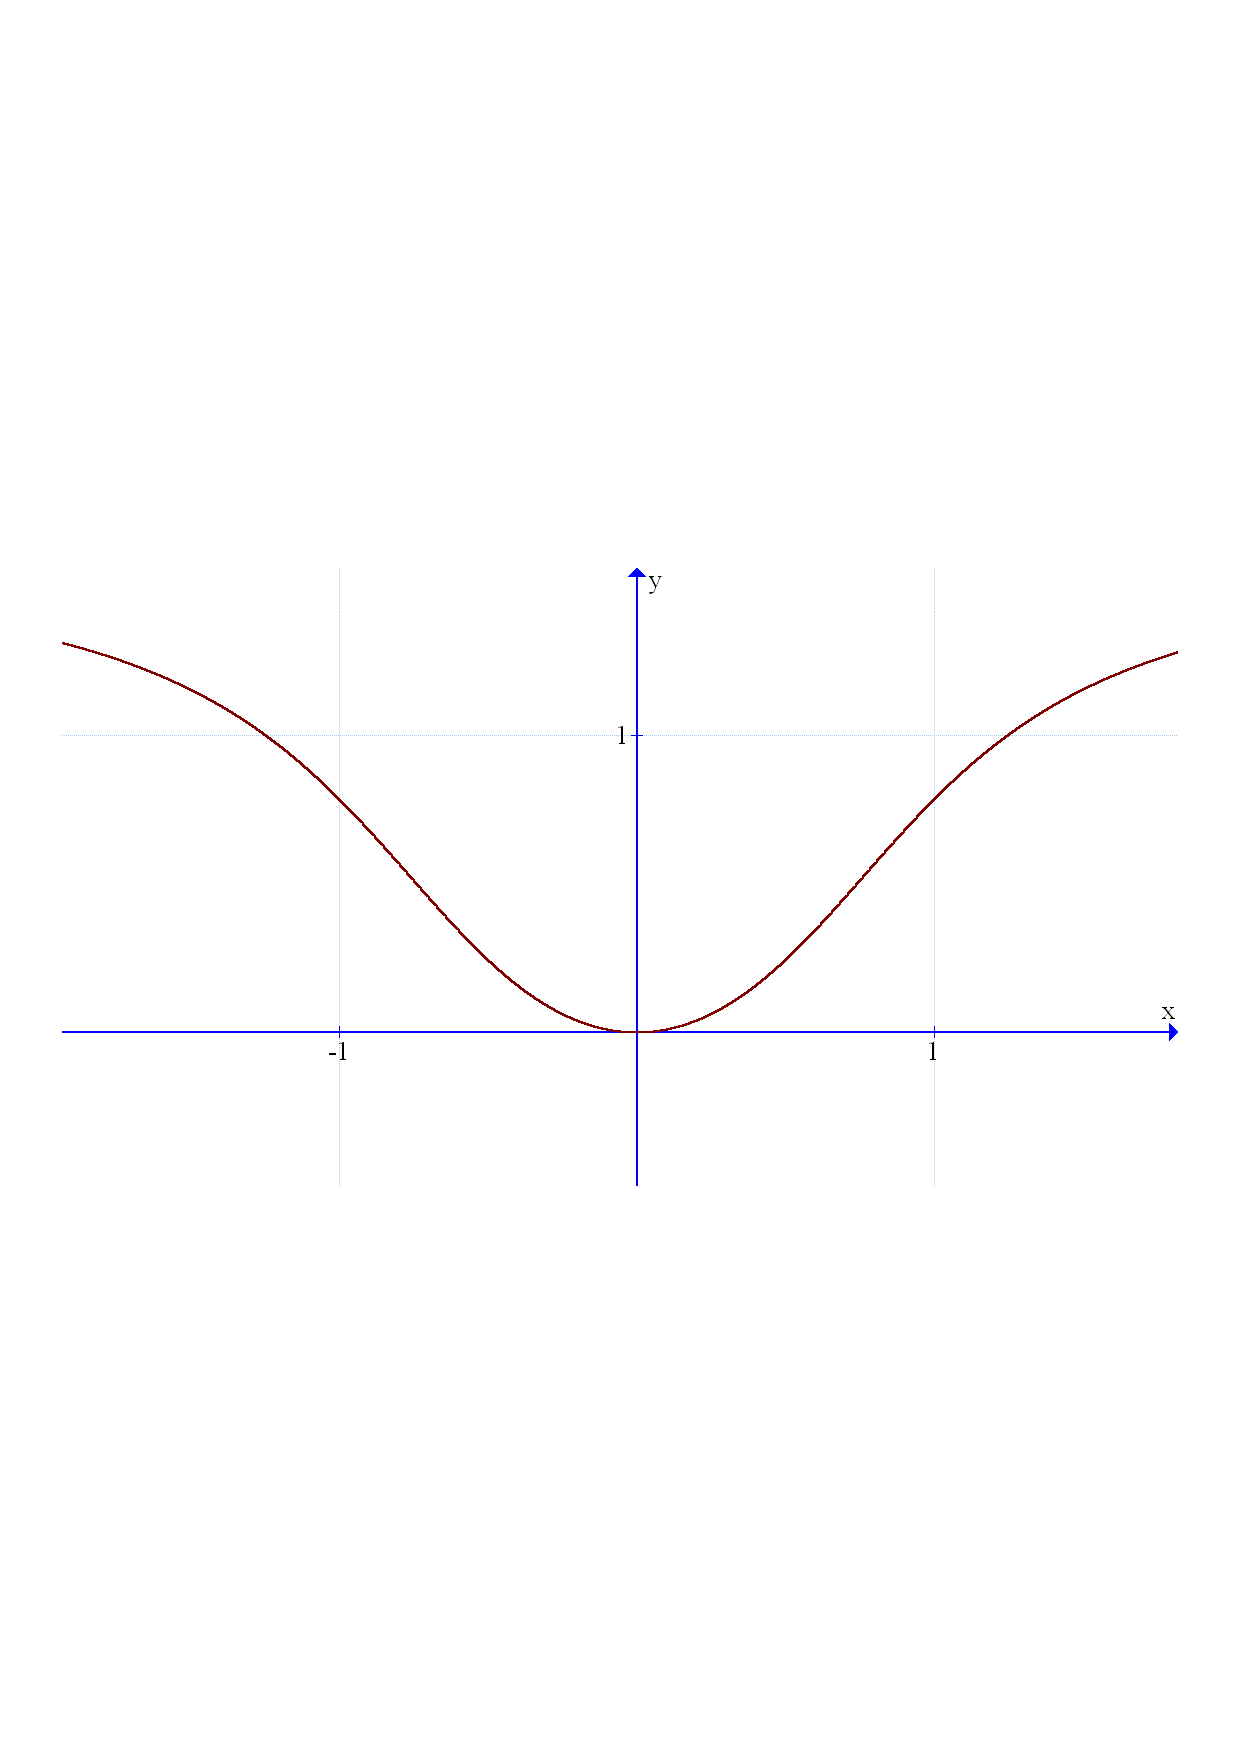
\includegraphics[scale=0.4]{atan.pdf}} \fi

\end{enumerate}

\item The screen at the front of a movie theater is 16 feet high and positioned 9 feet above eye level. How far away from the front of the room should you sit in order to have the ``best" view ? (HINT: Find the largest possible angle $\theta$ in diagram shown below.) 

\begin{center}
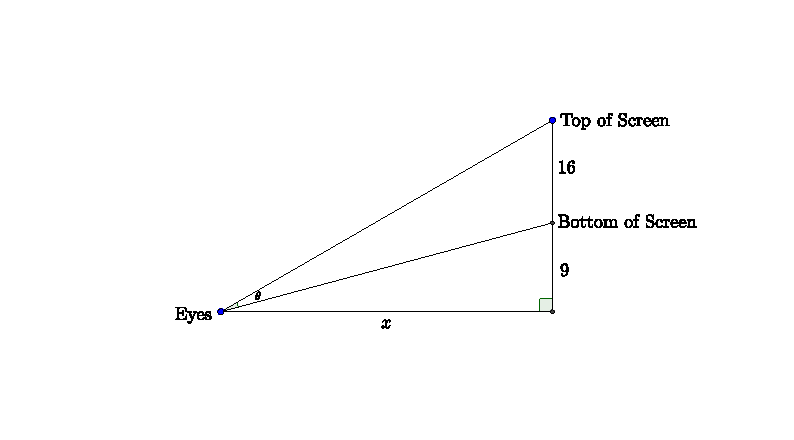
\includegraphics[scale=0.9]{screen.pdf}
\end{center}

\ifans\fbox{15 Feet}\fi

\item Find the area of the shaded region by adding together the area of the sector and the area of the triangle.

\begin{center}
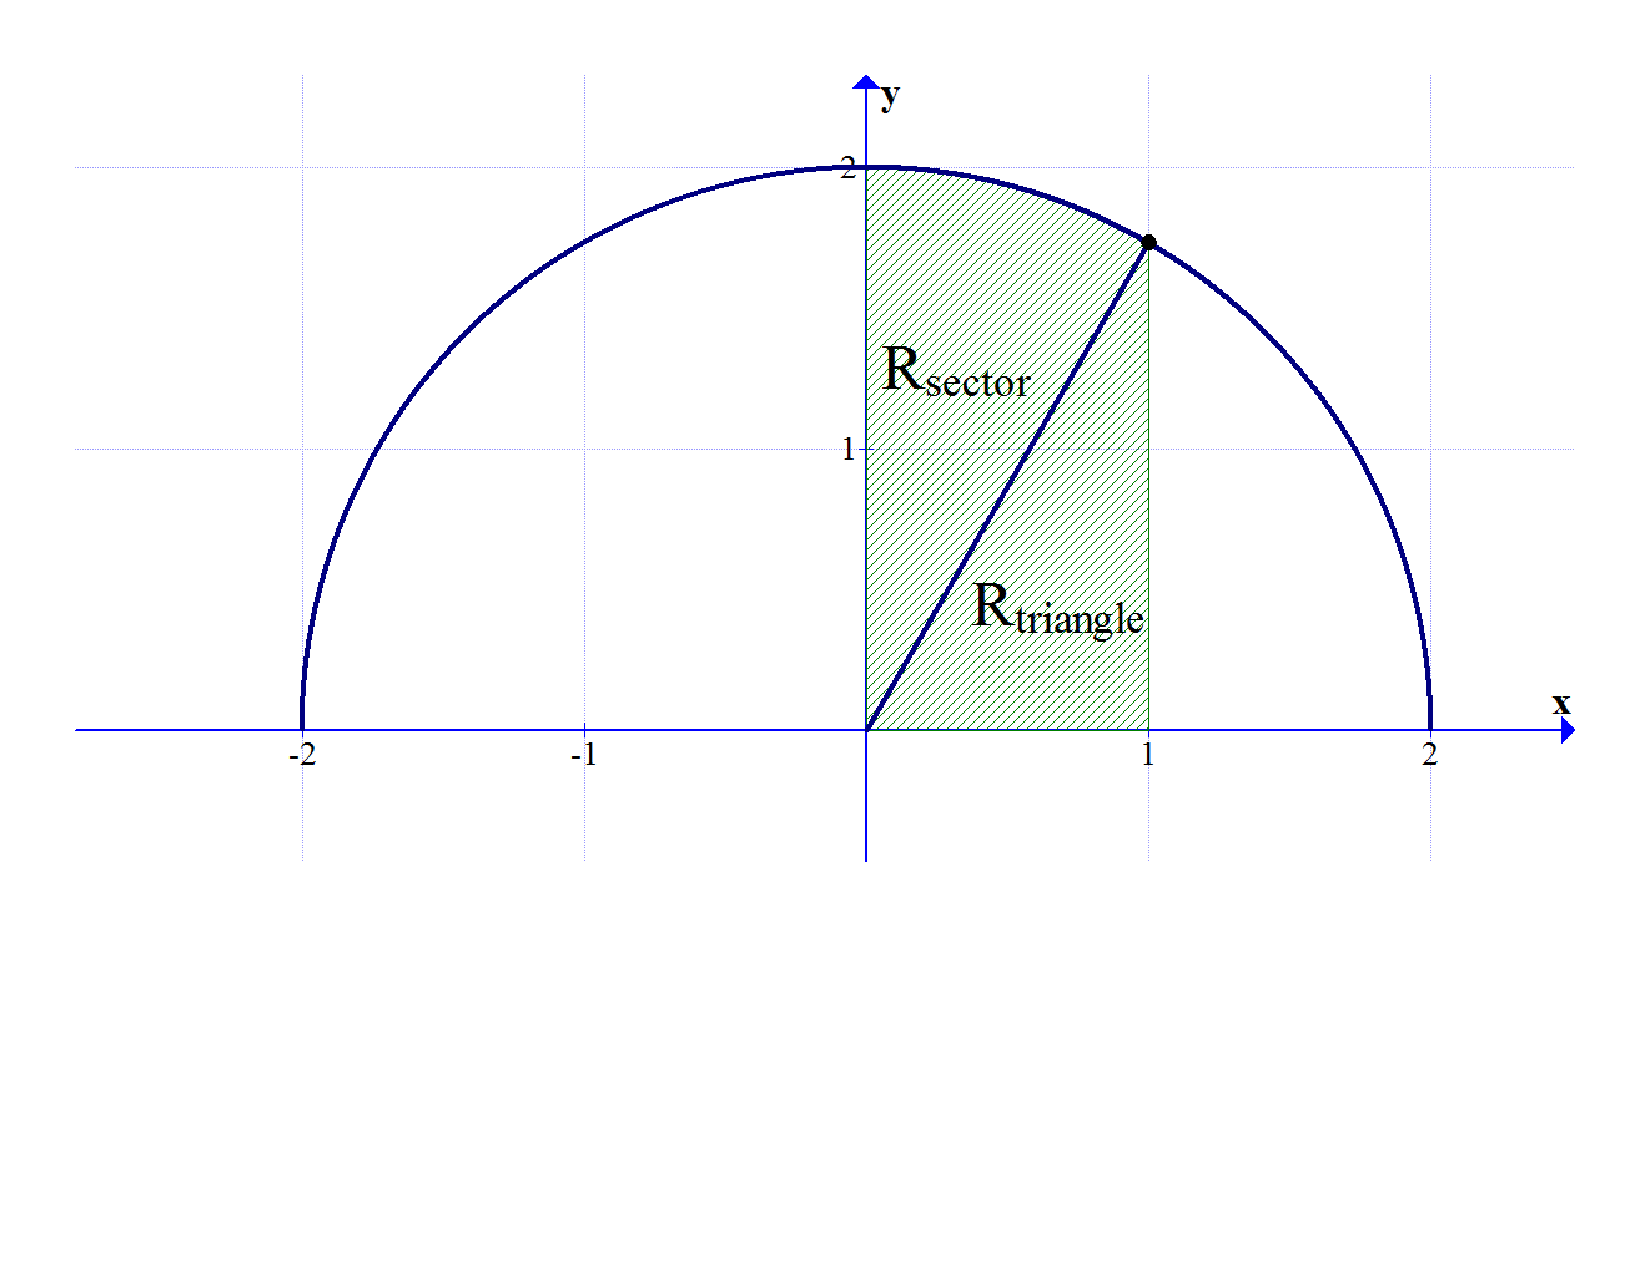
\includegraphics[scale=0.35]{area2.pdf}
\end{center}

\ifans{\fbox{\parbox{1\linewidth}{$Area of R_{\text{Triangle}}=\frac{1}{2}bh=\frac{1}{2}(1)\left(\sqrt{3}\right)=\frac{\sqrt{3}}{2}$; Area of $R_{\text{Sector}}=\frac{1}{2}r^2\theta=\frac{1}{2}(2)^2\left(\frac{\pi}{6}\right)=\frac{\pi}{3}$.  Thus, the total area is $A= \frac{\sqrt{3}}{2}+\frac{\pi}{3}$.}}} \fi

\end{enumerate}

\end{document}